\section{Implementation Strategy}
\label{sec:remplementation}
\subsection*{Methodology}
\label{sec:methodology}
As this work was to  be done in group, we have to develop a framework so everyone could work and share their code independently.
\begin{itemize}
    \item Heterogeneous environments: several operating systems (linux, windows, macOS), various platforms (local laptop training, Kaggle Kernels notebook, remote machines at Ecole Polytechnique). On every platform, data has to be acessible and experiments results have to be stored in a way they can be retrieved. We used the Kaggle dataset feature to  host the raw dataset aswell as the preprocessed data.
    \item Privacy: as not sharing code was among the rules of the challenge, our source code remained private on GitHub (\textit{which made cloning operations even trickier when using Kaggle kernels}).
    \item Reproducibility: all our experiments are reproducible (source code tracking under git, local and cloud storage of experiments results using ~\href{https://wandb.ai/molecule-nlp-altegrad-23/molecule-nlp}{Weights and biases}).
\end{itemize}
An experiment is defined by a unique identifier and the instanciation of a model (tokenization method, architecture of the LLM and GNN), the configuration of an  optimizer and training hyper parameters. At inference time, we're using this unique identifier so we can safely instantiate a network and reload the weights (\textit{trained model are by construction compatible with inference. This avoids the risk of having a `.pth` weight file without knowning which architecture to use to reload it.}).
We wrote a framework which takes and solves all these constraints at once and allows to focus on training models.


\subsection*{Training conditions}
\label{sec:training conditions}
To setup the training loop, we started on a single NVIDIA GeForce RTX 2080 GPU with 6Gb of RAM. This was enough to make sure we could train.



\subsection*{Preliminary study}
\label{sec:preliminary study}
We first started with by simple models based on the base GCN (3 graph convolution layers followed by a global pooling layer and 2 layers MLP). Instead of fine tuning all parameter, we first started by freezing the LLM parameters. Although simple, this idea intuivitely has many advantages for traing:
\begin{itemize}
    \item We discard the huge memory cost of training a LLM (memory issues not only come from storing the weigths on the GPU but all the optimizers variables during backpropagation). The idea could have been pushed further by pre-computing the text embeddings and storing them on disk. 
    \item Intuivitely, freezing the LLM parameters should make the training more stable as the LLM embeddings acts as a kind of anchor that the GNN shall match.
\end{itemize}
Unfortunately, training achieves low accuracy although the number of parameters to train is lightweight. We added an "adapter" module which is simply a MLP which will adapt by projecting the text represention into a more adapted space which can match with the graph.
We also browsed Hugging Face to find models that could be dedicated to scientific-specific language processing. The Sci-Bert\cite{scibert} model improvements were two-fold during this preliminary study: a tokenizer dedicated to a scientific corpus is by nature more suited for scientific texts... here atom and molecule names.

Increasing the GNN size improves accuracy.

\begin{table*}[h]
    \centering
    \begin{tabular}{|c|c|c|c|c|}
    \hline
    \textbf{Experiment ID} & \textbf{Model Size} & \textbf{LLM} & \textbf{GNN} & \textbf{LRAP} \\ \hline
    101         & 593k                & Frozen Distill-Bert           & Base 3 layer GCN       & 18.7\%      \\ \hline
    106         & 964k                & Frozen Distill-Bert + Adapter & Base 3 layer GCN       & 26.8\%      \\ \hline
    114         & 2.125M              & Frozen Distill-Bert + Adapter & Big 5 layer GCN        & 31.6\%      \\ \hline
    112         & 964k                & Frozen Sci-Bert + Adapter     & Base 3 layer GCN       & 36.7\%      \\ \hline
    113         & 2.125M              & Frozen Sci-Bert + Adapter     & Big 5 layer GCN        & 39.8\%      \\ \hline
    65          & 66.9M               & Trainable Bert                & Base 3 layer GCN       & 63.5\%      \\ \hline
    400         & 110M                & Trainable Sci-Bert            & Base 3 layer GCN       & 66\%        \\ \hline
    \end{tabular}
    \caption{Base Models Specifications and Performances}
    \label{tab:preliminary_study_metrics}
\end{table*}

\begin{figure*}
    \centering
    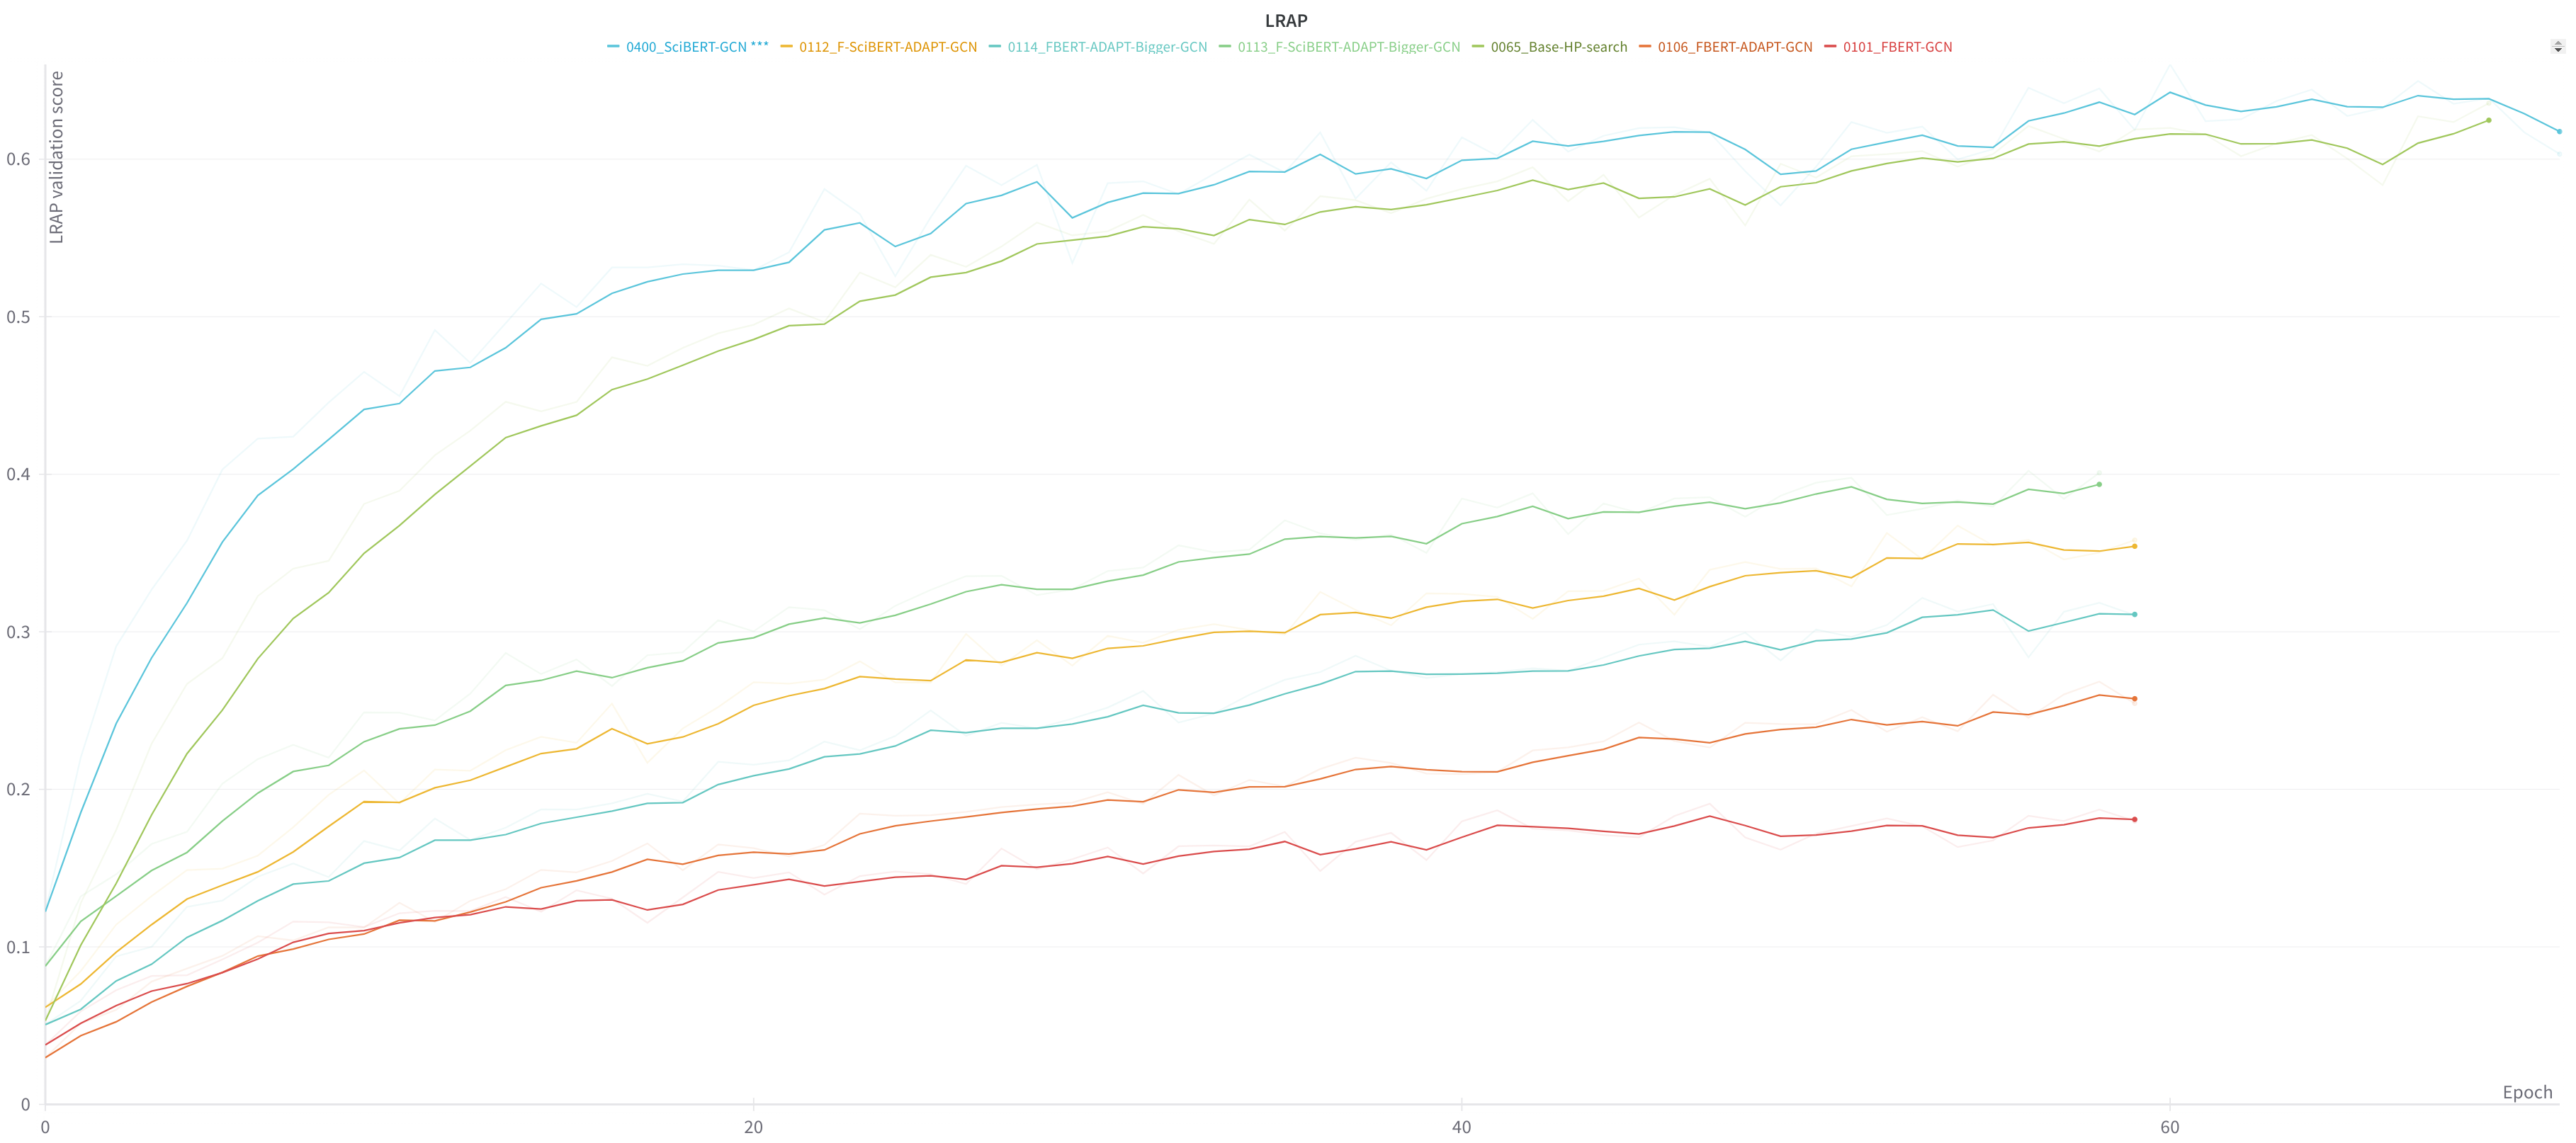
\includegraphics[width=1.\textwidth]{figures/preliminary_study.png}
    \caption{Training curves for the preliminary study.}
    \label{fig:preliminary_study_curves}
\end{figure*}
